\section{Basic concepts}



\begin{frame}
	%
	\frametitle{Environment declaration}
	%
	\begin{itemize}
		%
		\item template file for floating figures: \\
			\begin{center}
				\url{./Sources/template__floating_figure_declaration.tex}
			\end{center}
		%
		\vspace{1cm}
		%
		\item template file for non floating figures: \\
			\begin{center}
				\url{./Sources/template__non_floating_figure_declaration.tex}
			\end{center}
		%
	\end{itemize}
	%
\end{frame}









\begin{frame}
	%
	\frametitle{First main objects: nodes}
	%
	Main properties:
	%
	\begin{itemize}
		\item they are labelled (in order to be referenced)
		\item they can be placed everywhere
		\item you can write \LaTeX\ code inside them
		\item can be \emph{fully} customized
	\end{itemize}
	%
	\vspace{1cm}
	%
	(example file: \url{./Sources/basic_concepts__nodes_examples.tex})
	%
	\begin{figure}[!htb]
\begin{center}
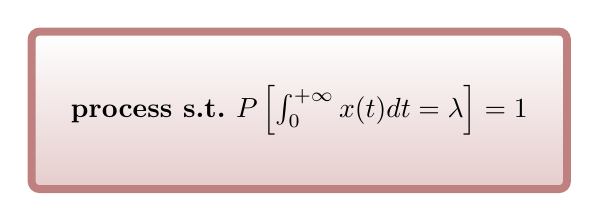
\begin{tikzpicture}
[
	xscale	= 1,	% to scale horizontally everything but the text
	yscale	= 1,	% to scale vertically everything but the text
]

\node
(nProcessNode)							% name of the node
[										% properties of the node:
	shape			= rectangle,		% shape
	rounded corners	= 0.1cm,			% roundness of the corners
	minimum height	= 2cm,				% | minimum size
	minimum width	= 6cm,				% |
	line width		= 0.1cm,			% thickness of the border
	draw			= red!50!black!50,	% colour of the border
	top color		= white,			% | filling colors
	bottom color	= red!50!black!20,	% |
	font			= \bfseries,		% used font
	inner xsep		= 0.5cm,			% minimum distance btw text and borders along x dimension
	inner ysep		= 0.5cm				% minimum distance btw text and borders along y dimension
]
{process s.t.\ $\mathbb{P} \left[ \int_{0}^{+\infty} x(t) dt = \lambda \right] = 1$}; % DON'T FORGET THE SEMICOLON!!

\end{tikzpicture}
\end{center}
\end{figure}

	%
\end{frame}





\begin{frame}
	%
	\frametitle{Second main objects: paths}
	%
	Main properties:
	%
	\begin{itemize}
		\item can be drawn everywhere - connect everything
		\item can have text along them
		\item can be \emph{fully} customized
	\end{itemize}
	%
	\vspace{1cm}
	%
	(example file: \url{./Sources/basic_concepts__paths_examples.tex})
	%
	\begin{figure}[!htb]
\begin{center}
\begin{tikzpicture}
[
	xscale	= 1,	% to scale horizontally everything but the text
	yscale	= 1,	% to scale vertically everything but the text
]

\draw
[
	->,										% kind of line
	rounded corners		= 0.4cm,			% behavior of the corners
	color				= blue!80!white,	%
	line width			= 0.1cm,			%
	dash pattern		= on 0.1cm    off 0.2cm    on 0.5cm    off 0.3cm,
	%
	postaction			=					% after having drawn the line ...
	{										%
		decorate,							% decorate it
		decoration		=					% with which decoration?
		{
			text along path,				% with some text...
			text			= {try to do this automatically in other ways 8-)}, % ...(this text)...
			text color		= blue!30!white	% ...of this color
		}
	}
]
(0cm,0cm) -- (1cm,1cm) -- (3cm,0cm) -- (8cm,0cm); % DON'T FORGET THE SEMICOLON!!

\end{tikzpicture}
\end{center}
\end{figure}

	%
\end{frame}





\begin{frame}
	%
	\frametitle{Well, not all can be done in a single presentation$\ldots$}
	%
	\begin{center}
	\begin{tikzpicture}
		%
		\node [WarningTextStyle]
		{and the coordinates specification??};
		%
	\end{tikzpicture}
	\end{center}
	%
	too time consuming to be fully explained! We'll use only:
	%
	\begin{itemize}
		%
		\item absolute coordinates (like \texttt{at (1.3cm, 2.1cm)})
		%
		\item relative coordinates (like \texttt{above this guy, left of this other})
		%
	\end{itemize}
	%
	\uncover<2->
	{
		\begin{center}
		\begin{tikzpicture}
			%
			\node [scope fading = east]
			{\large{again: \alert{take a look a the manual$\ldots\ldots\ldots$}}};
			%
		\end{tikzpicture}
		\end{center}
	}
	%
\end{frame}

